\documentclass[tikz,border=10pt]{standalone}
\usepackage{tikz}
\usetikzlibrary{shapes, arrows.meta, positioning, calc}

\begin{document}

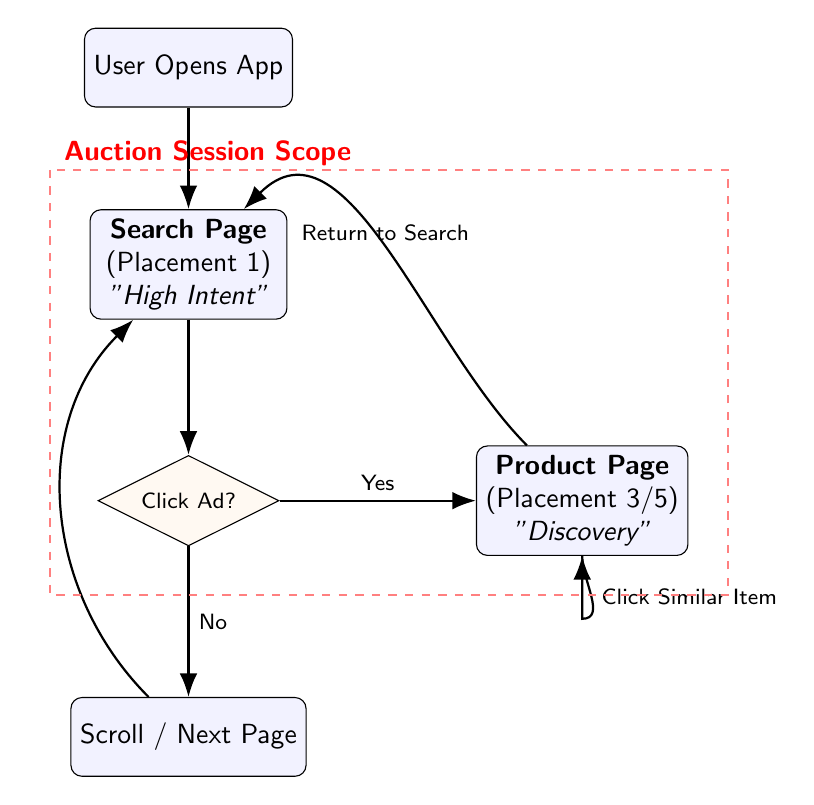
\begin{tikzpicture}[node distance=2.5cm, auto, >=stealth]
    % Styles
    \tikzstyle{state} = [rectangle, draw, rounded corners, minimum height=1cm, minimum width=2.5cm, align=center, fill=blue!5, font=\sffamily]
    \tikzstyle{decision} = [diamond, draw, align=center, aspect=2, fill=orange!5, font=\sffamily\footnotesize]
    \tikzstyle{arrow} = [draw, -{Latex[length=3mm]}, thick]
    \tikzstyle{label} = [midway, font=\footnotesize\sffamily]

    % Nodes
    \node[state] (start) {User Opens App};
    \node[state, below of=start] (search) {\textbf{Search Page} \\ (Placement 1) \\ \textit{"High Intent"}};
    \node[decision, below of=search, node distance=3cm] (click) {Click Ad?};
    \node[state, right of=click, node distance=5cm] (product) {\textbf{Product Page} \\ (Placement 3/5) \\ \textit{"Discovery"}};
    \node[state, below of=click, node distance=3cm] (scroll) {Scroll / Next Page};
    
    % Edges
    \draw[arrow] (start) -- (search);
    \draw[arrow] (search) -- (click);
    \draw[arrow] (click) -- node[label, above] {Yes} (product);
    \draw[arrow] (click) -- node[label, right] {No} (scroll);
    \draw[arrow] (scroll) to [out=135,in=225] (search);
    \draw[arrow] (product) to [out=135,in=45] node[label, above] {Return to Search} (search);
    \draw[arrow] (product) to [out=270,in=0] node[label, right] {Click Similar Item} +(0,-1.5) -| (product);

    % Scope Box
    \draw[dashed, red!50, thick] ($(search.north west)+(-0.5,0.5)$) rectangle ($(product.south east)+(0.5,-0.5)$);
    \node[red, font=\bfseries\sffamily] at ($(search.north west)+(1.5,0.7)$) {Auction Session Scope};

\end{tikzpicture}

\end{document}
